\documentclass[UTF8]{ctexart}
\usepackage{cite}
\usepackage{url}
\usepackage{amsfonts}    
\usepackage{amsmath}      
\usepackage{amssymb}
\usepackage{listings}
\usepackage{graphicx}
\usepackage{subfigure}
\usepackage{xspace}
\usepackage{float} 

\title{读书笔记(三)}
\author{黄怀宇}
\date{\today}
\lstdefinestyle{styleM}{language=matlab}
\lstdefinestyle{stylePy}{language=python}

\begin{document}
\maketitle

\section{算法评价}
\subsection{应用场景}
首先,要明确 判别异常的标准。

是否存在客观的标签,是判别异常标准的前提。而客观的标签取决人类的判断,也就是人类主观的意识。

对于人类用 眼睛-右脑 可以明显区分物品的情境,可以用 人为手工加标签的方式 制作 用来评价异常检测算法的数据集,常用的评价指标有 TP, TN, FP, FN,我们将它称为 情境1。 对于 不同人对同一组待检测的物品区分结果 可能有差异的情境,手工添加标签的方式 不能达到 前一种情境的效果,我们称其为 情境2。对于情境1,例子是 人类可以很轻松地区分 一张人和一张狗的图片。对于情境2,例子是 人类对判断一张狗和人图片 morphing 后的结果存在争议。

所以,在实际应用场景中,要人为判断所在场景更适合用情境1(有标签) 还是情境2(无标签)。对于网络流量的异常检测可以认为是情境2(无标签),此类对异常的定义与分类不是非此即彼,需要人为选定“尺度”。

尺度,可以定义为判断异常的严厉程度,是一个可调的参数,适用于不同的需求。比如对于 图一 的 DBSCAN 算法的第三个测试数据集,如果把尺度定义地大一点,则图中上半部分的黑点可以和蓝点归为一类,如果尺度定义的小一点,则其右上角凸起的矩形区域应如 SpectralClustering 算法。

对于情境2而言,评价算法的标准应是 其分类结果是否符合大多数人的直观感受,比如 对于 Birch 算法的第一个数据集,大多数人的直观感受是里面一个圈唯物一类,外面一个圈为一类,而 Birch 算法没有做到这一点,所以此算法在此类数据集上的分类是比较失败的。以此为评价标准,对于分类得比较成功的算法,有SpectralClustering 和 DBSCAN,对于算法的评价应用人类的评价标准,比如,前者对于第四个数据集欠拟合,绿色类左端不应该归为蓝色类;且它对于第六个数据集过拟合,三块颜色应为一类;后者对于第四个数据集在其边缘上略微过拟合,是当前所有列出的算法中表现最好的。

\subsection{测试数据集}

\begin{figure}[H] %H为当前位置,!htb为忽略美学标准,htbp为浮动图形
\centering %图片居中
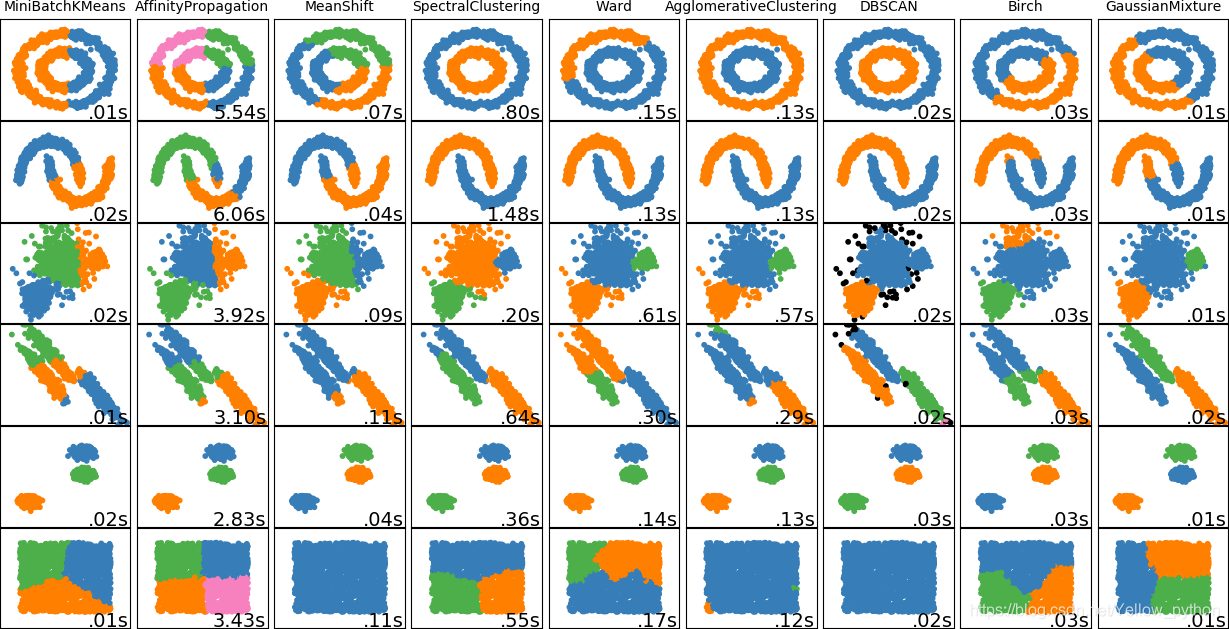
\includegraphics[width=1.0\textwidth]{cite_dataset.png} %插入图片,[]中设置图片大小,{}中是图片文件名
\caption{Fully benchmark} %最终文档中希望显示的图片标题
\protect\cite{link8}
% \label{Fig.main2} %用于文内引用的标签
\end{figure}

\subsection{直观上判断}

SpectralClustering 对于 第四个 有欠拟合,对第六个过拟合。
DBSCAN 对于第四个在边缘上略微过拟合,是所列出算法中表现最好的。

\subsection{划分异常检测结果评价的模块划分}
这也是之后工作的目录与步骤。
    \subsubsection{数据集可视化}
    可以灵活地添加新型的数据集,在添加之前可清楚地看到数据集标准的样子,也就是 数据集预览。

    \subsubsection{数据的制作}
    制作新的数据聚集样式,尽可能得使其标准化。
    % 手绘数据,自动生成

    \subsubsection{基于传统的评价方式}
    此方式对应情境1。
    % 因为 经验主义 目前尚未在学术界被广泛接受,理性主义 在学术圈仍然占据主导地位,所以不得不用数据说话,在 主观判断 的基础上加上 科学的数据分析,也可以与后面的调研相结合,看看 情境1 与 情境2 相关性大不大。

    根据聚类后的数据和原始数据的差异,计算 TP, TN, FP, FN,定量评价异常检测算法的好坏。

    \subsubsection{基于人类主观判断的评价方式}
    此方式对应情境2。

    只给被调研者聚类后的图像,给定几个指标,要求被调研者评价该聚类的好坏。

\section{数据集可视化}
创建一个叫 datasetPreview 的模块
\begin{lstlisting}[style=stylePy]
import numpy as np, matplotlib.pyplot as mp
from sklearn.preprocessing import StandardScaler
from itertools import cycle, islice

def showDataset(name, dataset):
    X, y = dataset

    # use it when y == None
    # if y == None:
    #     y = [0] * X.shape[0]

    X = StandardScaler().fit_transform(X)
    mp.title(name, size=10)
    colors = np.array(list(islice(
        cycle(['#377eb8', '#ff7f00', '#4daf4a',
                '#f781bf', '#a65628', '#984ea3',
                '#999999', '#e41a1c', '#dede00']),
                int(max(y) + 1))))
    colors = np.append(colors, ["#000000"]) 
    mp.scatter(X[:, 0], X[:, 1], s=10, 
      color=colors[y])
    mp.xlim(-2.5, 2.5)
    mp.ylim(-2.5, 2.5)
    mp.xticks(())
    mp.yticks(())
    mp.show()


if __name__ == '__main__':
    pass
\end{lstlisting}

使用模块
\begin{lstlisting}[style=stylePy]
import numpy as np
from sklearn import cluster, datasets, mixture
from sklearn.neighbors import kneighbors_graph
import datasetPreview as dp

if __name__ == '__main__':
    """
    1. data
    2. tag used for judge
    (
        array([xx, xx], [xx, xx], ... , [xx, xx]),  
        array(0|1, 0|1, ... , 0|1)                  
    )
    """
    np.random.seed(0)  
    n_samples = 1500
    noisy_circles = datasets.make_circles(
        n_samples=n_samples, factor=.5, noise=.05)

    dp.showDataset('preview', noisy_circles)
\end{lstlisting}

\begin{figure}[ht]
\centering
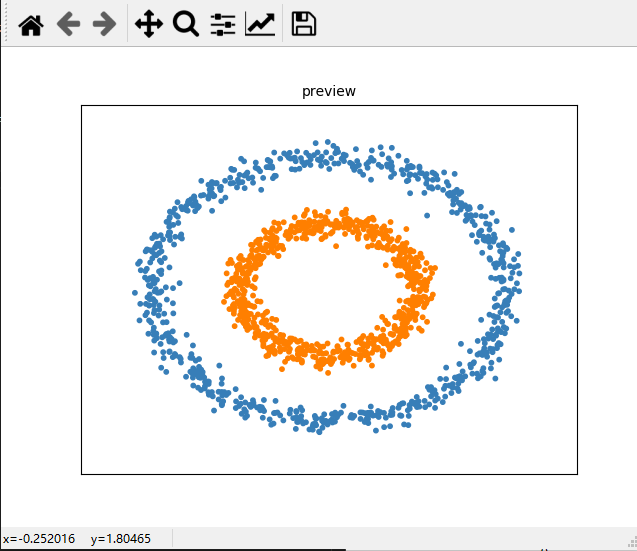
\includegraphics[scale=0.5]{dp.png}
\caption{datasetPreview module}
\end{figure}


\section{数据集的制作}
\subsection{sklearn 提供的数据生成器}
使用 sklearn.datasets 中的典型数据
%\subsection{手动绘制}
% 获取鼠标位置,染色的同时输出坐标,去重,标准化,去重

\subsection{其它数学方法生成}
方法一:
\begin{lstlisting}[style=stylePy]
import numpy as np
from sklearn import cluster, datasets, mixture
import datasetPreview as dp

np.random.seed(0)  
n_samples = 1500
no_structure = np.random.rand(n_samples, 2), None
dp.showDataset('preview', no_structure)
\end{lstlisting}

\begin{figure}[ht]
\centering
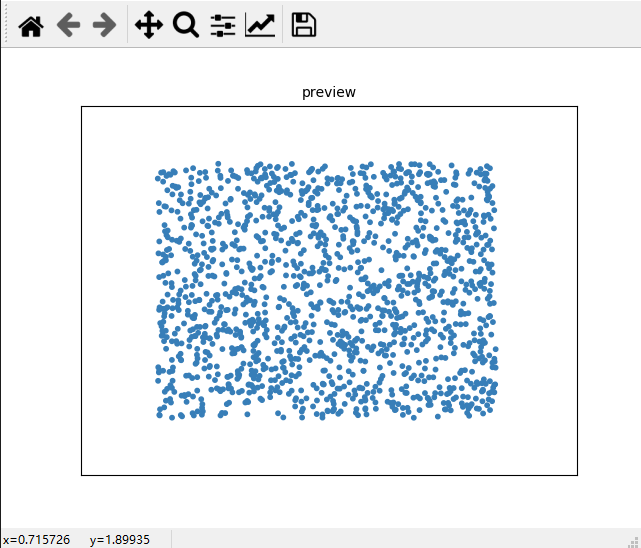
\includegraphics[scale=0.5]{otherDataset.png}
\caption{datasetPreview module}
\end{figure}

方法二(变换原来的数据):
\begin{lstlisting}[style=stylePy]
import numpy as np
from sklearn import cluster, datasets, mixture
import datasetPreview as dp

np.random.seed(0)  
n_samples = 1500
random_state = 170
X, y = datasets.make_blobs(
  n_samples=n_samples, random_state=random_state)
transformation = [[0.6, -0.6], [-0.4, 0.8]]
X_aniso = np.dot(X, transformation)
aniso = (X_aniso, y)
dp.showDataset('preview', aniso)
\end{lstlisting}

\begin{figure}[ht]
\centering
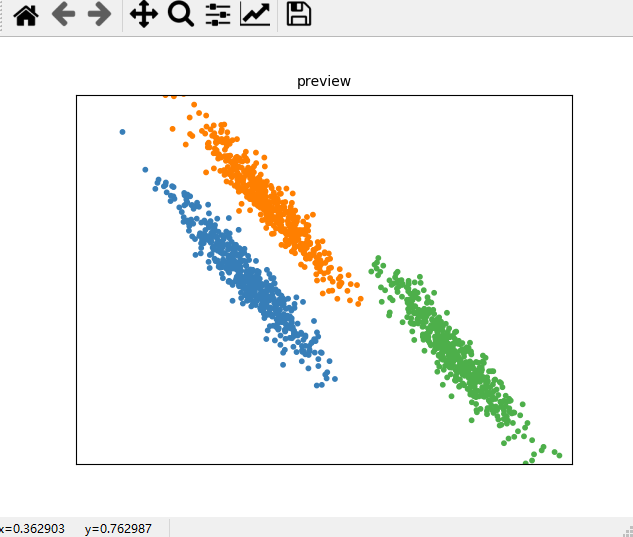
\includegraphics[scale=0.5]{aniso.png}
\caption{datasetPreview module}
\end{figure}

\subsection{系统设计中使用的数据}
在实际应用中,需要用到现实的数据用作 benchmark,我对数据集的需求(或者说我研究的应用场景)是:

1. 适用于无监督异常检测的情境

2. 数据尽量和流量相关

3. 数据维数尽可能小。

在网上搜寻后,发现 The Numenta Anomaly Benchmark (NAB)和 Anomaly Detection Toolkit (ADTK) 符合要求。

值得注意的是,它们的数据是基于时间序列的,

\section{两种评价方式}
\subsection{需求分析}
系统输入的是一群无标签的含异常的数据,可以是 .csv 文件,数据进入系统后,数据先可视化;然后根据数据集的模式(形状),人工选择合适的算法;然后开始计算,计算完成后,得到的数据不但有对各个点的分类情况,还有对本次分类结果的可视化和评价,评价的参数用 The Numenta Anomaly Benchmark (NAB) 的 Standard Profile 来表示。% 数据集模式分析 人工|自动

而正常的数据是多维的,可视化无法达到预期的效果,所以,系统要解决的问题是 根据已有的数据集,预测新输入的数据异常数据是否为异常数据。

\subsection{基于科学数据的评价方式}
这里采用 The Numenta Anomaly Benchmark (NAB) 项目的指标。以 The Numenta Anomaly Benchmark (NAB) 中的 Scoreboard 为准。

precesion:查准率,即在检索后返回的结果中,真正正确的个数占整个结果的比例。

recall:查全率,即在检索结果中真正正确的个数 占整个数据集(检索到的和未检索到的)中真正正确个数的比例。

FN:False Negative,被判定为负样本,但事实上是正样本。

FP:False Positive,被判定为正样本,但事实上是负样本。

TN:True Negative,被判定为负样本,事实上也是负样本。

TP:True Positive,被判定为正样本,事实上也是证样本。

precesion = TP/(TP+FP) 即,检索结果中,都是你认为应该为正的样本(第二个字母都是P),但是其中有你判断正确的和判断错误的(第一个字母有T ,F)。

recall = TP/(TP+FN)即,检索结果中,你判断为正的样本也确实为正的,以及那些没在检索结果中被你判断为负但是事实上是正的(FN)。

\begin{figure}[ht]
\centering
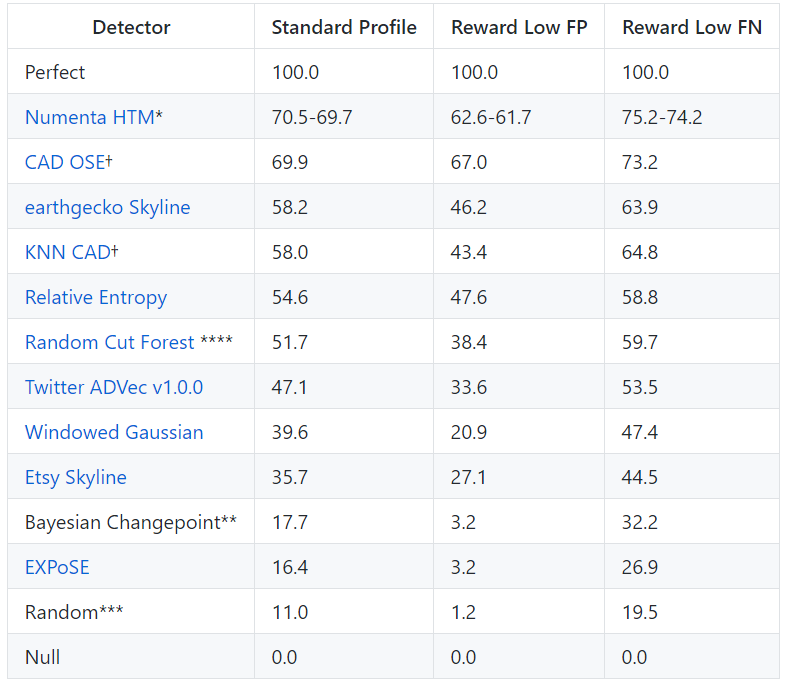
\includegraphics[scale=0.5]{NAB-benchmark.png}
\caption{datasetPreview module}
\end{figure}

\subsection{基于人类主观判断的评价方式}
由于此系统已经可视化了分类前后数据的模式,所以人类可以直观地判断数据分类的情况。这个方式需要做一些调研工作,可以最后做。

\section{系统设计}
% 还没想好

\section{复现算法与可视化}
代码实现
\begin{lstlisting}[style=stylePy]
from time import time
import numpy as np, matplotlib.pyplot as mp
from sklearn import cluster, datasets, mixture
from sklearn.neighbors import kneighbors_graph
from sklearn.preprocessing import StandardScaler  
from itertools import cycle, islice

np.random.seed(0)  
n_samples = 1500
noisy_circles = datasets.make_circles(
  n_samples=n_samples, factor=.5, noise=.05)
noisy_moons = datasets.make_moons(n_samples=n_samples, noise=.05)
blobs = datasets.make_blobs(n_samples=n_samples, random_state=8)
no_structure = np.random.rand(n_samples, 2), None
random_state = 170
X, y = datasets.make_blobs(n_samples=n_samples, 
  random_state=random_state)
transformation = [[0.6, -0.6], [-0.4, 0.8]]
X_aniso = np.dot(X, transformation)
aniso = (X_aniso, y)
varied = datasets.make_blobs(n_samples=n_samples,
                            cluster_std=[1.0, 2.5, 0.5],
                            random_state=random_state)

mp.figure(figsize=(9 * 2 + 3, 12.5))
mp.subplots_adjust(left=.02, right=.98, bottom=.001, top=.96,
  wspace=.05, hspace=.01)
plot_num = 1

default_base = {'quantile': .3, 
                'eps': .3,  
                'damping': .9,  
                'preference': -200,
                'n_neighbors': 10,
                'n_clusters': 3}

datasets = [
    (noisy_circles, {'damping': .77, 'preference': -240, 
      'quantile': .2, 'n_clusters': 2}),
    (noisy_moons, {'damping': .75, 'preference': -220, 
      'n_clusters': 2}),
    (varied, {'eps': .18, 'n_neighbors': 2}),
    (aniso, {'eps': .15, 'n_neighbors': 2}),
    (blobs, {}),
    (no_structure, {})]

for i_dataset, (dataset, algo_params) in enumerate(datasets):
    params = default_base.copy()
    params.update(algo_params)
    X, y = dataset
    X = StandardScaler().fit_transform(X)
    bandwidth = cluster.estimate_bandwidth(X, 
      quantile=params['quantile'])
    connectivity = kneighbors_graph(
        X, n_neighbors=params['n_neighbors'], include_self=False)
    connectivity = 0.5 * (connectivity + connectivity.T)

    ms = cluster.MeanShift(bandwidth=bandwidth, bin_seeding=True)
    two_means = cluster.MiniBatchKMeans(n_clusters=params['n_clusters'])
    ward = cluster.AgglomerativeClustering(
        n_clusters=params['n_clusters'], linkage='ward', 
          connectivity=connectivity)
    spectral = cluster.SpectralClustering(
        n_clusters=params['n_clusters'], eigen_solver='arpack', 
          affinity="nearest_neighbors")
    dbscan = cluster.DBSCAN(eps=params['eps'])
    affinity_propagation = cluster.AffinityPropagation(
        damping=params['damping'], preference=params['preference'])
    average_linkage = cluster.AgglomerativeClustering(
        linkage="average", affinity="cityblock",
        n_clusters=params['n_clusters'], connectivity=connectivity)
    # Balanced Iterative Reducing and Clustering Using Hierarchies
    birch = cluster.Birch(n_clusters=params['n_clusters'])
    gmm = mixture.GaussianMixture(
        n_components=params['n_clusters'], covariance_type='full')
    clustering_algorithms = (
        ('MiniBatchKMeans', two_means),
        ('AffinityPropagation', affinity_propagation),
        ('MeanShift', ms),
        ('SpectralClustering', spectral),
        ('Ward', ward),
        ('AgglomerativeClustering', average_linkage),
        ('DBSCAN', dbscan),
        ('Birch', birch),
        ('GaussianMixture', gmm)
    )
    for name, algorithm in clustering_algorithms:
        t0 = time()
        algorithm.fit(X)
        t1 = time()
        if hasattr(algorithm, 'labels_'):
            y_pred = algorithm.labels_.astype(np.int)
        else:
            y_pred = algorithm.predict(X)
        mp.subplot(len(datasets), len(clustering_algorithms), plot_num)
        if i_dataset == 0: 
            mp.title(name, size=10)
        colors = np.array(list(islice(cycle(['#377eb8', '#ff7f00', '#4daf4a',
                                                '#f781bf', '#a65628', '#984ea3',
                                                '#999999', '#e41a1c', '#dede00']),
                                        int(max(y_pred) + 1))))
        colors = np.append(colors, ["#000000"])  
        mp.scatter(X[:, 0], X[:, 1], s=10, color=colors[y_pred])

        mp.xlim(-2.5, 2.5)
        mp.ylim(-2.5, 2.5)
        mp.xticks(())
        mp.yticks(())
        mp.text(.99, .01, ('%.2fs' % (t1 - t0)).lstrip('0'),
                transform=mp.gca().transAxes, size=14, horizontalalignment='right')
        plot_num += 1
mp.show()
\end{lstlisting}

运行结果
\begin{figure}[ht]
\centering
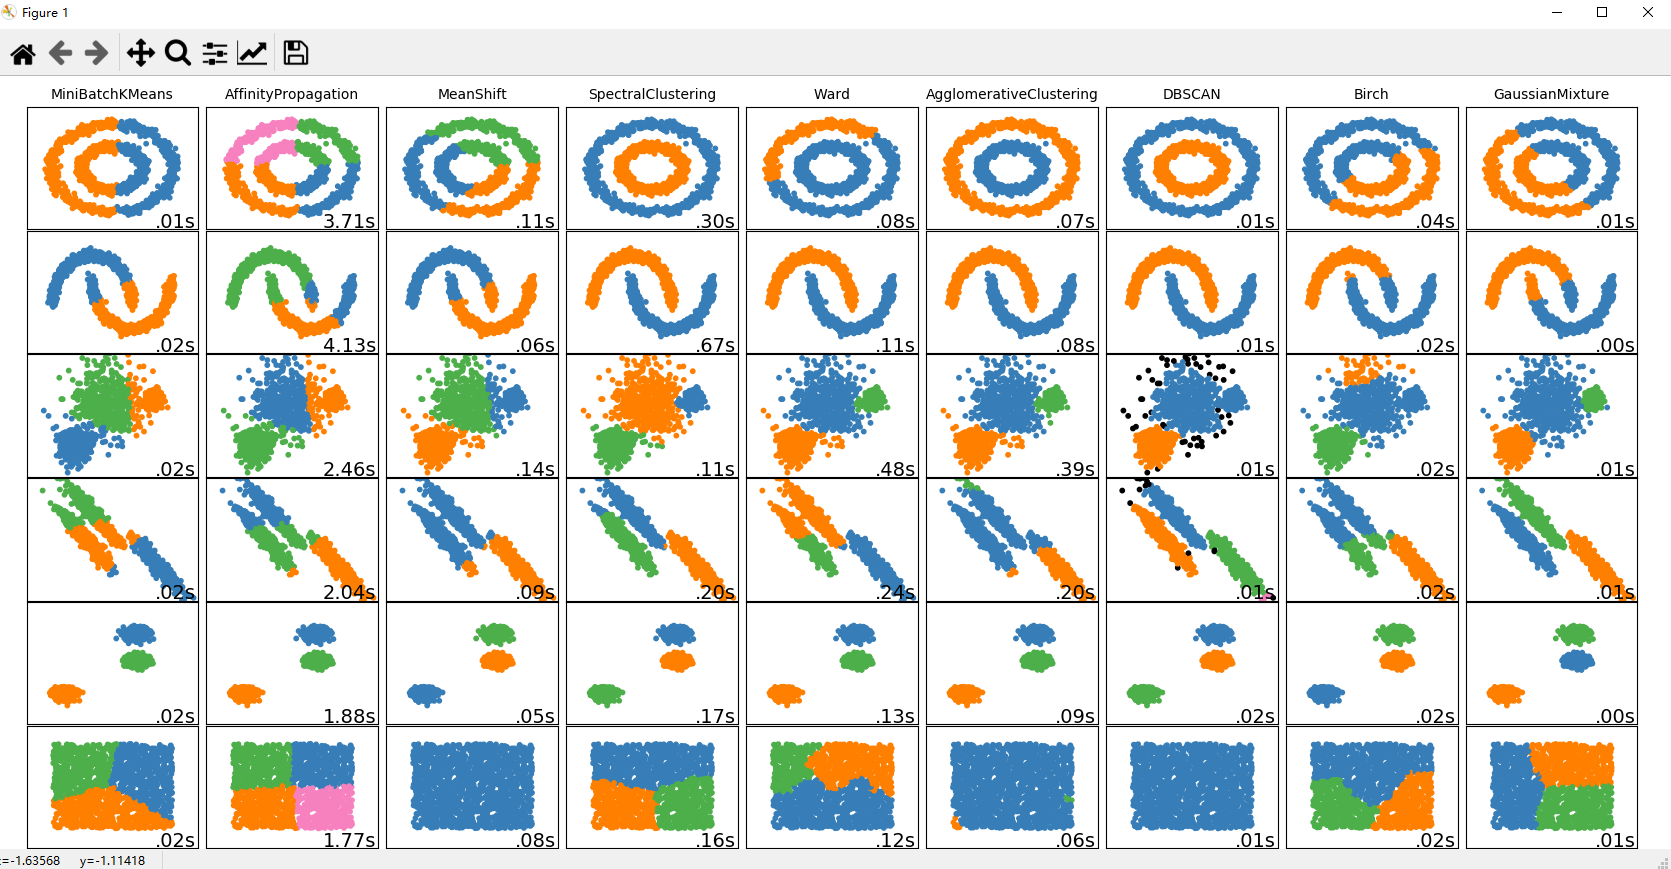
\includegraphics[scale=0.4]{resultBenchmarkpic.png}
\caption{datasetPreview module}
\end{figure}


\section{判断时间序列异常检测的方法}
    \subsection{异常类型}
        \subsubsection{点异常}
        离散点、孤立点、异常值
        \subsubsection{上下文异常}
        值无异常,但是在上下文环境中呈现异常
        \subsubsection{集合异常}
        单点无异常,但子集相对于全集呈现异常
    \subsection{异常检测}
        \subsubsection{直接检测}
        针对点异常,直接定位离群点
        \subsubsection{间接检测}
        上下文或集合异常先转化成点异常,然后再求解
    \subsection{算法概览}
        \subsubsection{STL分解}
        不是机器学习方法,不选择。
        \subsubsection{分类和回归树}
        分为有监督和无监督。选择无监督模型。流行的库是 xgboost
        \subsubsection{ARIMA}
        整合移动平均自回归模型。它的思路是过去的若干数据点加上某个随机变量(通常是白噪声)可以预测下一个数据点。预测数据点可以进一步用来生成新预测,以此类推。显然,它的效果是让信号变得更平滑。应用这一方法的难点在于你需要通过Box-Jenkins方法选择差异数、自回归数、预测误差系数。处理新信号时应该创建新ARIMA模型。另一个麻烦是对信号取差值后得到的信号应该是停滞的。也就是说,信号不应取决于时间,这是一个显著的限制。创建一个适应离群点的模型,基于t统计量看它是否比原模型更好地拟合数据,这就可以实现异常检测。\cite{link11}
        \subsubsection{神经网络}
        神经网络有两种应用方式:监督学习和无监督学习。由于我们处理的是时序数据,最合适的神经网络类型是LSTM。如果构建得当,这种循环神经网络可以建模时序中最复杂的依赖关系,包括高层季节性依赖。这一方法在处理耦合的多个时序数据时非常有用。这一领域仍在研究之中,创建时序模型需要花很多功夫。不过,如果你成功的话,你可能取得突出的精确度。\cite{link11}

    \subsection{选用无监督机器学习异常检测算法的优势}
        \subsubsection{各算法优缺点的比较}
        STL分解的优点在于其简单性和强大性。它可以处理很多不同的情况,并且仍然可以直观地解释所有异常情况,它主要用于检测附加异常值。要检测电平变化,您可以分析一些滚动平均值信号,而不是原始信号。这种方法的弊端在于调整选项的刚性。您可以调整的只是使用显着性水平的置信区间,无法正常运作的典型情况是信号的特征发生了巨大变化,例如,您要跟踪网站上对公众关闭然后突然打开的用户。在这种情况下,您应该分别跟踪启动期间之前和之后发生的异常。

        分类和回归树的优势在于,它在任何程度上都不受信号结构的束缚,并且您可以引入许多特征参数来进行学习并获得复杂的模型。缺点是,越来越多的功能可以很快开始影响您的计算性能。在这种情况下,您应该有意识地选择功能。

        ARIMA(整合移动平均自回归模型)是一个设计得非常简单的方法,但仍然足够强大,可以预测信号并指出其中的异常值。它的思路是过去的若干数据点加上某个随机变量(通常是白噪声)可以预测下一个数据点。预测数据点可以进一步用来生成新预测,以此类推。显然,它的效果是让信号变得更平滑。应用这一方法的难点在于你需要通过Box-Jenkins方法选择差异数、自回归数、预测误差系数。处理新信号时应该创建新ARIMA模型。另一个麻烦是对信号取差值后得到的信号应该是停滞的。也就是说,信号不应取决于时间,这是一个显著的限制。创建一个适应离群点的模型,基于t统计量看它是否比原模型更好地拟合数据,这就可以实现异常检测。

        指数平滑技术和ARIMA方法非常类似。基本指数模型等价于ARIMA (0, 1, 1)模型。从异常检测的角度来说,我们最感兴趣的是Holt-Winters季节性方法。你需要定义季节性周期,比如一周、一月、一年。万一你需要追踪多种季节性周期,比如同时追踪周和年,你应该选择其中的一种。通常是选择最短的周期,比如,在周和年之间选择周。很明显,这是该方法的一个缺陷,会大大影响预测范围。和STL或CART一样,通过统计学检验可以实现异常检测。

        神经网络和CART的情形类似,神经网络有两种应用方式:监督学习和无监督学习。由于我们处理的是时序数据,最合适的神经网络类型是LSTM。如果构建得当,这种循环神经网络可以建模时序中最复杂的依赖关系,包括高层季节性依赖。这一方法在处理耦合的多个时序数据时非常有用。这一领域仍在研究之中,创建时序模型需要花很多功夫。不过,如果你成功的话,你可能取得突出的精确度。\cite{link11}


\bibliography{cites.bib}
\bibliographystyle{ieeetr}

\end{document}